\documentclass[a4paper,11pt]{article}
\usepackage[T1]{fontenc}
\usepackage[utf8]{inputenc}
\usepackage{lmodern}
\usepackage{amsmath}
\usepackage{amsfonts}
\usepackage{amssymb}
\usepackage{amsthm}
\usepackage{graphicx}
\usepackage{color}
\usepackage{url}
\usepackage{textcomp}
\DeclareMathOperator*{\argmax}{argmax}
\DeclareMathOperator*{\argmin}{argmin}

\title{Value Iteration}
\author{Joshua Tsang}
\date{\today}

\begin{document}

\maketitle
\tableofcontents

\section{Foundational Concepts}

It is instructive intially discuss the foundational concepts in Markov Decision Problems (MDP) and Reinforcement Learning (RL).  Consider the problem shown in Figure \ref{fig:1d-grid-world-problem-statement} where an agent is located in one of the grid positions.

\begin{figure}
    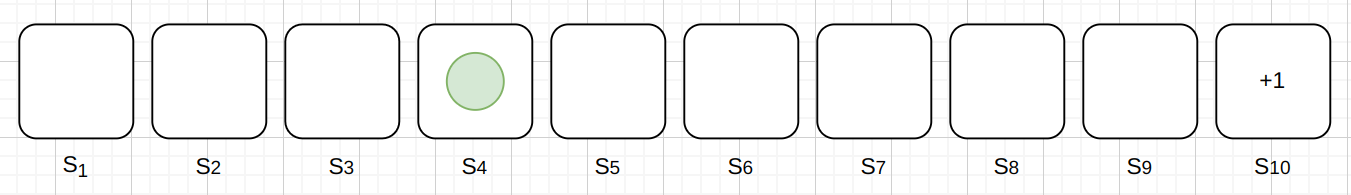
\includegraphics[width=\textwidth]{images/1d-grid-world-problem-statement.png}
    \caption{1D Grid World MDP with an assigned reward of $+10$ in state $s_{10}$, termed the terminal state.  The agent currently sits in state $s_4$ and the goal of the problem is for the agent to take actions to maximise its reward.  At each state other than the terminal state, there is a negative reward of $-1$.  Drawn with draw.io and saved in Google Drive as 1D\_grid\_world.drawio.}
    \label{fig:1d-grid-world-problem-statement}
\end{figure}


\begin{itemize}
    \item State Space and State: The finite State Space of a system is denoted $S$ where a state $s$ denotes a certain configuration of the system i.e. $s \in S$.  For example, in Figure \ref{fig:1d-grid-world-problem-statement} the agent is currently in state $s_4$, with the neighbouring states, $\{s'\}$, being $s_3$ and $s_5$.
    \item Actions: For each state, $s_i$, that the system resides in a set of available actions, $\{a_k\}$, can be taken that transition the system to another state, $s_j$.  For Figure \ref{fig:1d-grid-world-problem-statement} the available actions at state $s_4$ are \verb|(move left)| and \verb|(move right)|.  One could think of a graph where nodes are states and the edges are actions.
    \item Policy: A policy, denoted $\pi$, dictates the action to take for a given state.  It is often written as a function $\pi(s, a)$ where it is formally defined as:
    \begin{equation} \label{eqn:policy_formal_definition}
        \pi(s,a) = P(a=a|s=s)
    \end{equation}
    which is the probability of taking action $a$ given the system is in state $s$.  The goal of Reinforcement Learning is to learn the optimal policy $\pi(s,a)$ to maximise future rewards (explained next). As a foreshadow, policy functions are often expressed as an $\argmax_a$ as follows:
    \begin{equation} \label{eqn:value_iteration_foreshadow}
        \pi(s,a) = \argmax_a Q(s, a)
    \end{equation}
    i.e. an $\argmax$ over the available actions which returns the argument (action) that returns the maximum value for the quality function $Q$ (defined later).
    \item Reward: Numerical reward can be associated with certain states and actions, represented as $R_t$ for the current time step.  In the case of Figure \ref{fig:1d-grid-world-problem-statement}, there is a fixed reward of $+10$ at state $s_{10}$ and the other states have a reward of $-1$.  The goal of RL can be considered to be finding the sequence of actions that maximise the sum of rewards to achieve a sucessful episode i.e. the agent reaches the terminal state $s_{10}$.
    \item Episodes:  MDPs have the characteristic of being finite i.e. they end within a finite number of time steps, denoted $T$.  More specifically, an episode is a sequence of states, actions and rewards that start at some state and end in the terminal state.
    \item Return or "Future Gains":  Usually denoted $G_t$ it is the sum of rewards gained by the agent {\it after} time step $t$, define as:
    \begin{equation} \label{eqn:return_G_t}
        G_t = R_{t+1} + R_{t+2} + ... + R_{T}
    \end{equation}
    It is possible to introduce a discount rate $\gamma \in [0,1]$ that diminishes the rewards gained further in the future:
    \begin{equation} \label{eqn:return_G_t}
        G_t = R_{t+1} + \gamma R_{t+2} + \gamma^2 R_{t+2} + ... + \gamma^{T-1-t} R_{T}
    \end{equation}
    note how the power of $\gamma$ in the final term is $T-1-t$ and {\it not} $T$, a little thought makes this clear (for example, try write down $G_4$ where $T=8$).
\end{itemize}

\section{State Value Function, Bellman's Equation and the Principle of Optimality}

An important concept in Reinforcement Learning is the State Value Function, $V(s)$.

Defining the quality function as:
\begin{equation} \label{eqn:quality_function_Q}
    Q(s,a) = \sum_{s'} P(s'|s,a) \left[ R(s',s,a) + \gamma V(s') \right]
\end{equation}
where $s'$ are the neighbouring states to the current state, $s$.


\section{Value Iteration}

Value iteration allows one to assign state values to each state through repeated, iterative application of the value function, and the optimal policy is extracted at the end.  



\begin{figure}
    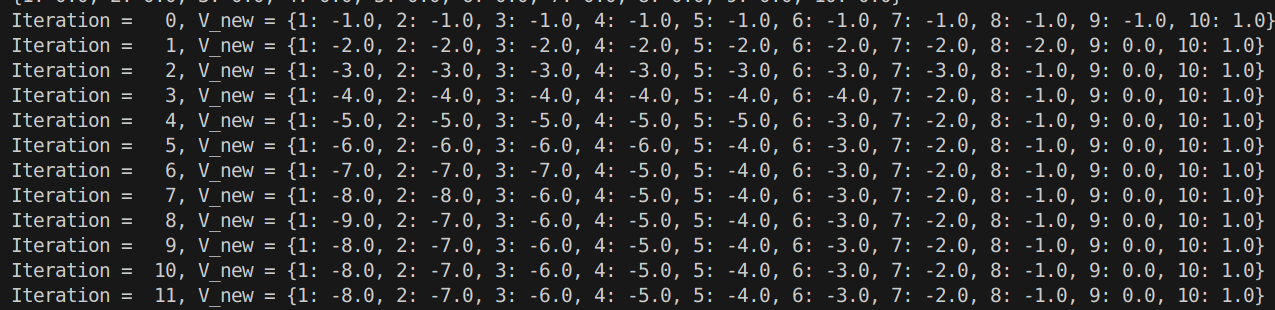
\includegraphics[width=\textwidth]{images/iters-of-value-iteration-1d-grid-world-code-output.png}
    \caption{Iterations of the value iteration algorithm.}
    \label{fig:iters-of-value-iteration-1d-grid-world-code-output}
\end{figure}


\section{Policy Iteration}

\end{document}